\section{Experiments and Results}
\label{sec:experiments}
%\vspace{-.2cm}
\subsection{Datasets}
\label{assec:Datasets}
We evaluate the MK-UNet's efficacy across six datasets covering four segmentation tasks, including breast cancer (BUSI \cite{al2020dataset}, 647 images: 437 benign and 210 malignant), polyp (ClinicDB \cite{bernal2015wm} with 612 images, and ColonDB \cite{vazquez2017benchmark} with 379 images), skin lesion (ISIC18 \cite{codella2019skin}, 2,594 images), and cell nuclei/structure segmentation (DSB18 \cite{caicedo2019nucleus} with 670 images, and EM \cite{cardona2010integrated} with 30 images). These datasets, collected from various imaging centers, offer a broad diversity in image characteristics, ensuring a comprehensive evaluation. An 80:10:10 train-val-test split was applied across all datasets and the DICE score of testset is reported.

%We evaluate the performance of our MK-UNet network, we conduct experiments across six datasets that belong to four medical image segmentation tasks. Specifically, we use BUSI \cite{al2020dataset} dataset for breast cancer segmentation. Following \cite{valanarasu2022unext}, we use 647 (437 benign and 210 malignant) images from this dataset. Besides, we use two polyp segmentation datasets: ClinicDB \cite{bernal2015wm} (612 images), and ColonDB \cite{vazquez2017benchmark} (379 images). These datasets contain images from different imaging centers/clinics, having greater diversity in image nature as well as size and shape of polyps. We consider ISIC18 \cite{codella2019skin} dataset (2,594 images) for skin lesion segmentation. DSB18 \cite{caicedo2019nucleus} (670 images) and EM \cite{cardona2010integrated} (30 images) datasets of biological imaging are used for cell nuclei/structure segmentation. We follow a train-val-test split of 80:10:10 in all the datasets.

%\vspace{-0.4cm}
\subsection{Implementation details}
\label{ssec:impl_details}
%We implement our network and conduct experiments using Pytorch 1.11.0 on a single NVIDIA RTX A6000 GPU with 48GB of memory. In the MKDC of our network, we set the multi-scale kernels $[1,3,5]$ through an ablation study. We use the parallel arrangement of depth-wise convolutions and the MK-UNet network with $[16,32,64,96,160]$ channels default in all experiments unless otherwise mentioned. Our models are trained using the AdamW optimizer \cite{loshchilov2017decoupled} with a learning rate and weight decay of $1e-4$. We train for 200 epochs with a batch size of 16, saving the best model based on the DICE score. We resize images to $256\times256$ for ISIC18 \cite{codella2018skin}, BUSI \cite{al2020dataset}, EM \cite{cardona2010integrated}, and DSB18 \cite{caicedo2019nucleus}. For ClinicDB \cite{bernal2015wm} and ColonDB \cite{vazquez2017benchmark}, images are resized to $352\times352$. We use a multi-scale \{0.75, 1.0, 1.25\} training strategy with a gradient clip limit of 0.5. We do not use any augmentation and optimize a combined weighted BinaryCrossEntropy (BCE) and weighted IoU loss function. 

Our networks are developed and evaluated using Pytorch 1.11.0, operating on a single NVIDIA RTX A6000 GPU equipped with 48GB of RAM.  We utilize multi-scale kernels $[1,3,5]$ within our MKDC, based on an ablation study. The architecture employs a series of parallel depth-wise convolutions in the MK-UNet network, standardizing on channel configurations of $[16,32,64,96,160]$ across all experiments, unless specified otherwise. Model optimization is achieved via the AdamW \cite{loshchilov2017decoupled} optimizer with both learning rate and weight decay set to $1e-4$. Training spans over 200 epochs with batches of 16, during which we save the model achieving the highest DICE score. 

Image dimensions are set to $256\times256$ pixels for BUSI \cite{al2020dataset}, ISIC18 \cite{codella2018skin}, EM \cite{cardona2010integrated}, and DSB18 \cite{caicedo2019nucleus} datasets, while for ClinicDB \cite{bernal2015wm} and ColonDB \cite{vazquez2017benchmark}, the resolution is adjusted to $352\times352$ pixels. We utilize a multi-scale training approach, with scales of \{0.75, 1.0, 1.25\}, and enforce gradient clipping at 0.5. We do not apply any form of augmentation and use a hybrid loss function that combines (1:1) weighted BinaryCrossEntropy (BCE) with a weighted Intersection over Union (IoU) loss.

%Following \cite{rahman2023cascade}, we resize images to $224\times224$, employ random rotation and flipping as data augmentation, and optimize the combined Cross-entropy (0.3) and DICE (0.7) loss for Synapse multi-organ and ACDC datasets. 
%We use a batch size of 6 and train each model for maximum of 300 epochs. We use the input resolution of $224 \times 224$ for PVT-GCASCADE and ($256\times256$, $224\times224$) for MERIT-GCASCADE. We apply random rotation and flipping for data augmentation. The combined weighted Cross-entropy (0.3) and DICE (0.7) loss are utilized as the loss function.

%\textbf{ACDC dataset.} For the ACDC dataset, we train each model for a maximum of 150 epochs with a batch size of 12. We set the input resolution as $224 \times 224$ for PVT-GCASCADE and ($256\times256$, $224\times224$) for MERIT-GCASCADE. We apply random flipping and rotation for data augmentation. We optimize the combined weighted Cross-entropy (0.3) and DICE (0.7) loss function.

%\textbf{Polyp datasets.} We resize the image to $352 \times 352$ and use a multi-scale \{0.75, 1.0, 1.25\} training strategy with a gradient clip limit of 0.5 like CASCADE \cite{Rahman_2023_WACV}. We use a batch size of 4 and train each model a maximum of 200 epochs. We optimize the combined weighted BinaryCrossEntropy (BCE) and weighted IoU loss function.

%\textbf{ISIC2018 dataset:} We resize the images into $384\times384$ resolution. Then, we train our model for 200 epochs with a batch size of 4 and a gradient clip of 0.5. We optimize the combined weighted BCE and weighted IoU loss function.
\begin{table*}[t]
%\vspace{-0.3cm}
%\vspace{-0.4cm}
\begin{center}
\begin{adjustbox}{width=0.88\textwidth}
\begin{tabular}{l|c|r|r|r|r|r|rr|rr|r}
\toprule
\multirow{2}{*}{Network} & \multirow{2}{*}{Pretrain} & \multirow{1}{*}{\#Params} & \multirow{1}{*}{FLOPs} & \multirow{1}{*}{Throughput} & \multirow{2}{*}{BUSI} &  \multirow{2}{*}{ISIC18} & \multicolumn{2}{c|}{Polyp} & \multicolumn{2}{c|}{Cell} & \multirow{2}{*}{Avg.}\\
\cline{8-11}
& & (M) & (G) & (/s) & & & Clinic & Colon & DSB18 & EM & \\
\midrule
UNet \cite{ronneberger2015u} & No & 34.53M & 65.53G & 119.03 & 74.04 & 86.67 & 91.43 & 83.95 & 92.23 & 95.36 & 87.28 \\
%ResUNet \cite{zhang2018road} & \textcolor{blue}{No} & 62.74M & 94.56G & 74.12 & 86.75 &  91.46 & 84.02 & 92.16 & 95.32 &  87.31 \\
UNet++ \cite{zhou2018unet++} & No & 9.16M & 34.65G & 136.98 & 74.76 & 87.46 & 91.52 & 87.88 & 91.97 & 95.38 & 88.16 \\
AttnUNet \cite{oktay2018attention} & No & 34.88M & 66.64G & 108.68 & 74.48 & 87.05 & 91.50 & 86.46 & 92.22 & 95.45 & 87.86 \\
DeepLabv3+ \cite{chen2017deeplab} & Yes & 39.76M & 14.92G & 128.20 & 76.81 & 88.64 & 92.46 & 89.86 & 92.14 & 94.96 & 89.15 \\
PraNet \cite{fan2020pranet} & Yes & 32.55M & 6.93G & 64.10 & 75.14 & 88.46 & 91.71 & 89.16 & 89.89 & 92.37 & 87.79 \\
UACANet \cite{kim2021uacanet} & Yes & 69.16M & 31.51G & 43.28 & 76.96 & 88.72 & 93.29 & 89.76 & 88.86 & 89.28 & 87.81 \\
TransUNet \cite{chen2021transunet} & Yes & 105.32M & 38.52G & 65.35 & 78.01 & 89.04 & 93.18  & 89.97 & 92.04 & 95.27 & 89.59 \\
SwinUNet \cite{cao2021swin} & Yes & 27.17M  & 6.2G & 80.64 & 77.38 & 88.66 & 92.42 & 89.07 & 91.03 & 94.47 & 88.84 \\
%ACC-UNet \cite{ibtehaz2023acc} & \textcolor{blue}{No} & 16.8M & 38.0G & 77.02 & 88.57 & 92.56 & 89.13 & 90.05 & 94.67 & 88.67 \\
%\textcolor{blue}{DeformableLKA \cite{azad2024beyond}} & \textcolor{blue}{No} & \textcolor{blue}{102.76M} & \textcolor{blue}{26.03G} & \textcolor{blue}{15.08} & \textcolor{blue}{74.62} & \textcolor{blue}{88.17} & \textcolor{blue}{91.05} & \textcolor{blue}{85.93} & \textcolor{blue}{92.12} & \textcolor{blue}{94.45} & \textcolor{blue}{87.72} \\
%\hline
Rolling-UNet-S \cite{liu2024rolling} & No & 1.78M &  2.1G & 57.14 & 76.38 &  87.35 & 90.23 & 82.48 & 92.50 & 95.23 & 87.36\\
MedT \cite{valanarasu2021medical} & No & 1.57M & 1.95G & 8.40 & 69.23 & 86.78 & 83.44 & 68.90 & 92.28 & 93.87 & 82.42 \\
UNeXt \cite{valanarasu2022unext} & No & 1.47M & 0.57G & 172.41 & 74.71 & 87.78 & 90.20 & 83.84 & 86.01 & 93.81 & 86.06 \\
CMUNeXt \cite{tang2023cmunext} & No & 0.418M & 1.09G & \textbf{175.43} & 77.34 & 87.51 & 92.82 & 83.85 & 92.58 & 95.38 & 88.25 \\
EGE-UNet \cite{ruan2023ege} & No &  0.054M &  0.072G & 101.01 & 71.34 &  86.95 & 84.76 & 76.03 & 90.10 & 93.76 & 83.82 \\
UltraLight\_VM\_UNet \cite{wu2024ultralight} & No & 0.050M & \textbf{0.060G} & 98.03 & 72.31 & 87.85  & 87.11  & 80.06 & 91.88 & 93.96 & 85.53 \\
\midrule
\textbf{MK-UNet-T (Ours)} & No & \textbf{0.027M} & 0.062G & 140.85 & 75.64 & 88.19 & 91.26 & 85.03 & 92.38 & 94.69 &  87.87 \\
\textbf{MK-UNet-S (Ours)} & No & 0.093M & 0.125G & 139.42 & 77.26 & 88.57 & 92.31 & 88.78 & 92.45 & 95.22 &  89.10 \\
\textbf{MK-UNet (Ours)} & No & 0.316M & 0.314G & 138.89 & 78.04 & 88.74 & 93.48 & 90.01 & 92.71 & 95.52 &  89.75 \\
\textbf{MK-UNet-M (Ours)}    & No  & 1.15M  & 0.951G &  133.73 & 78.27 & 89.08 & 93.67 & 90.27 & 92.74 & 95.62 & 89.94 \\
\textbf{MK-UNet-L (Ours)}    & No    & 3.76M & 3.19G &  122.62 & \textbf{79.02} & \textbf{89.25} & \textbf{93.85} & \textbf{91.82} & \textbf{92.80} & \textbf{95.67} & \textbf{90.40} \\

%\method{}-M (\textbf{Ours}) & 1.15 & 0.951 & 77.87 & 89.28 & 93.35 & 89.87 & 92.70 & 95.62 &  \\
\bottomrule
\end{tabular}
\end{adjustbox}
\vspace{-0.2cm}
\caption{Results of binary (breast cancer, skin lesion, polyp, and cell) segmentation. We reproduce the results of SOTA methods using their publicly available implementations with our 80:10:10 train-val-test splits. FLOPs of all methods are reported for $256\times256$ inputs. The FLOPs of all methods for polyp segmentation with $352\times352$ inputs will be higher. We report DICE scores (\%) averaging over five runs, thus having 1-4\% standard deviations. $[C1, C2, C3, C4, C5]$ = MK-UNet-T $[4, 8, 16, 24, 32]$, MK-UNet-S $[8, 16, 32, 48, 80]$, MK-UNet $[16, 32, 64, 96, 160]$, MK-UNet-M $[32, 64, 128, 192, 320]$, and MK-UNet-L $[64, 128, 256, 384, 512]$. Best results are shown in \textbf{bold}.}
\label{tab:results_binary_mis}
\end{center}
\vspace{-0.5cm}
\end{table*}


%\vspace{-0.4cm}
\subsection{Results}
\label{ssec:results}
Table \ref{tab:results_binary_mis} and Fig. \ref{fig:dice_vs_params_flops} compare our MK-UNet with SOTA CNNs and transformers on six datasets of four binary medical segmentation tasks. Our MK-UNet achieves the top average DICE score of 89.75\%, while maintaining an ultra-lightweight footprint of only 0.316M \#Params and 0.314G \#FLOPs. Our MK-UNet-T with 0.027M \#Params and 0.062G \#FLOPs, outperforms the existing most tiny model EGE-UNet \cite{ruan2023ege} by on an average 5.93\% DICE score over six datasets. The multi-kernel depth-wise convolutions within our network, alongside local attention mechanisms, play a crucial role in these strong results. Our MK-UNet's performance on different datasets highlights its superior ability to balance accuracy with computational efficiency, setting a new benchmark for point-of-care diagnostics. The quantitative results of four different tasks are described next.

\subsubsection{Breast cancer segmentation}
We focus on breast cancer segmentation in ultrasound images using the BUSI dataset. Our MK-UNet model notably outperforms existing methods, achieving the highest DICE score of 78.04\% with remarkably low computational requirements. This achievement underscores the efficiency and effectiveness of our approach, particularly when compared against more complex models. For instance, TransUNet, despite having substantially more parameters (105.32M) and FLOPs (38.52G), achieves a lower DICE score of 78.01\%. Similarly, ACC-UNet, with its 16.8M parameters and 38.0G FLOPs, closely follows with a DICE score of 77.02\%. Additionally, compared to the computationally comparable model UNeXt, our MK-UNet demonstrates a significant improvement, surpassing it by a margin of 3.33\% with 4.7$\times$ fewer \#Params. %Our MK-UNet's performance on the BUSI dataset highlights its superior ability to balance accuracy with computational efficiency, setting a new benchmark in the field of point-of-care medical image segmentation.


\subsubsection{Skin lesion segmentation}
On the ISIC18 dataset for skin lesion segmentation, our MK-UNet network exhibits a commendable performance with a DICE score of 88.74\%. This result not only showcases our model's robustness, but also its capability to handle the complex variations present in skin lesion images. We note that TransUNet leads with a marginally higher score of 89.04\% but with a significantly higher cost (333$\times$ and 123$\times$ larger \#Params and \#FLOPs, respectively). Our MK-UNet achieves near-top performance while maintaining minimal computational requirements—merely 0.316M \#Params and 0.314G \#FLOPs. %This complete contrast in resource utilization without a substantial compromise in accuracy highlights MK-UNet's innovative design, making it an ideal solution for effective and efficient skin lesion segmentation task.

\subsubsection{Polyp segmentation}
\label{sssec:polyp_results}
In polyp segmentation on Clinic and Colon datasets, our MK-UNet model excels with leading scores of 93.48\% and 90.01\%, respectively, and with a remarkably low computational footprint. This performance surpasses notable competitors like DeepLabv3+ and ACC-UNet, which, despite their higher resource consumption, do not match MK-UNet's precision. Specifically, DeepLabv3+ reaches 92.46\% on Clinic and 89.86\% on Colon with 126$\times$ and 47.5$\times$ larger parameters and FLOPs, respectively, while ACC-UNet closely follows but still falls short. %MK-UNet's efficiency and accuracy in detecting polyps highlight its innovative design, setting new standards for resource-effective polyp segmentation without compromising on quality.

\subsubsection{Microscopic cell nuclei/structure segmentation}
For cell nuclei/structure segmentation on the DSB18 and EM datasets, our MK-UNet network demonstrates exceptional accuracy, achieving DICE scores of 92.71\% and 95.52\%, respectively. In contrast, other models like TransUNet and UNeXt, despite their heavy-weight design and higher computational demands, do not surpass MK-UNet's DICE score. For instance, TransUNet achieves lower scores of 92.04\% on DSB18 and 95.27\% on EM, while UNeXt falls 6.70\% behind MK-UNet.%, showcasing the efficiency and effectiveness of our model in cell segmentation tasks.

\begin{figure*}[t]
%\vspace{-.1cm}
\centering
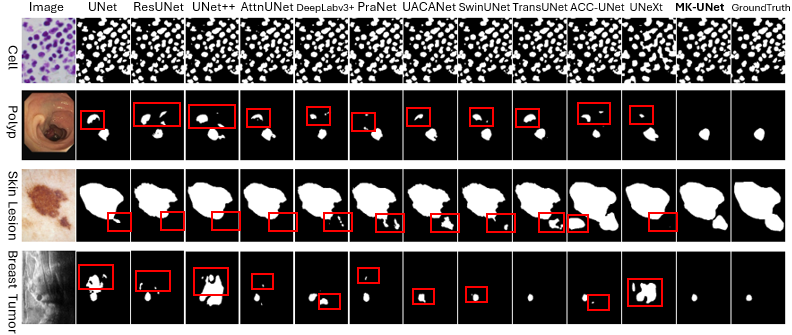
\includegraphics[width=0.95\textwidth]{sections/imgs/qualitative_results.png}
\vspace{-.2cm}
\caption{Qualitative results of our MK-UNet and SOTA methods. The incorrect segmented regions by different methods are highlighted using the red rectangular box.} 
\label{fig:qualitative}
\vspace{-.2cm}
\end{figure*}

\begin{table*}[t]
%\vspace{-.2cm}
\begin{center}
    %{\small{
    \begin{adjustbox}{width=0.75\textwidth}
\begin{tabular}{c|r|r|r|r|r|r|r|r}
\toprule
%\multicolumn{3}{c}{Components} & \multicolumn{2}{c}{\#FLOPs(G)} & \multicolumn{1}{c}{\#Params} & \multicolumn{1}{r}{Avg}  \\
Network     & \#Params & \#FLOPs & BUSI & Clinic & Colon & ISIC18 & DSB18 & EM                    \\
\midrule
Baseline UNeXt          & 1.47M & 0.57G & 74.71 &  90.20 & 83.84 &  87.78 & 86.01 & 93.81    \\
Redesigned Mobile UNet          & 0.271M     & 0.230G     & 72.41  & 90.90 & 84.15 & 87.20 & 90.52 & 94.87  \\
MKIR          & 0.306M    & 0.300G     & 74.74 & 92.63 & 86.46 & 88.22 & 92.40 & 95.31         \\
MKIR + GAG          & 0.310M     & 0.311G    & 74.98  & 91.97 & 86.56 & 88.34 & 92.67 & 95.48     \\
MKIR + MKIRA         & 0.311M    & 0.303G    &  76.61 & 92.64 & 89.40 &  88.56 & 92.64 & 95.37     \\
\textbf{MKIR + GAG + MKIRA (Ours)}        & 0.316M    & 0.314G    & \textbf{78.04} & \textbf{93.48} & \textbf{90.01} & \textbf{88.64} & \textbf{92.71} & \textbf{95.52}       \\
\bottomrule 
\end{tabular}
%}}
\end{adjustbox}
\end{center}
\vspace{-0.5cm}
\caption{Effect of different components of MK-UNet with \#channels = $[16,32,64,96,160]$ and $[1,3,5]$ kernels. UNeXt has \#channels = $[16,32,128,160,256]$. We design Mobile UNet following the structure of UNeXt network. However, we use the \#channels = $[16,32,64,96,160]$ and kernel size of $[3]$ with the original inverted residual block (IRB) in the Mobile UNet. We report the DICE scores (\%) averaging over five runs. Best results are shown in \textbf{bold}.}
\vspace{-0.4cm}
\label{tab:ablation_components}
\end{table*}


\begin{table*}[t]
%\vspace{-0.2cm}
%\vspace{-0.3cm}
\centering 
    {%\small{
\begin{adjustbox}{width=0.8\textwidth}
{\begin{tabular}{crrr|crrr}
\toprule
Convolution kernels & \#Params(M) & FLOPs(G) & DICE & Convolution kernels & \#Params(M) & FLOPs(G) & DICE\\
\midrule
$1\times1$           & 0.272 & 0.220 & 70.83 & $5\times5$           & 0.299 & 0.276 & 76.81 \\
$1\times1, 1\times1$         & 0.275 & 0.229 & 71.11 & $1\times1, 5\times5$         & 0.303 & 0.286 & 77.05 \\
$3\times3$           & 0.281 & 0.239 & 76.42 & $3\times3, 3\times3, 3\times3$       & 0.306 & 0.295 & 76.86 \\
$1\times1, 3\times3$         & 0.284 & 0.248 & 76.81 & $3\times3, 5\times5$         & 0.312 & 0.304 & 77.62 \\
$1\times1, 1\times1, 3\times3$       & 0.288 & 0.257 & 77.08 & \textbf{1$\times$1, 3$\times$3, 5$\times$5}       & 0.316 & 0.314 & \textbf{78.04} \\
$3\times3, 3\times3$         & 0.294 & 0.267 & 76.83 & $5\times5, 5\times5$         & 0.331 & 0.342 & 77.88 \\
$1\times1, 3\times3, 3\times3$       & 0.297 & 0.276 & 77.26 & $5\times5, 5\times5, 5\times5$       & 0.362 & 0.408 & 77.80 \\
%$3\times3, 5\times5, 7\times7$       & 0.371 & 0.426 & 77.63 \\
\bottomrule
\end{tabular}}
\end{adjustbox}
}%}
\vspace{-0.2cm}
\caption{Effect of multiple kernels in the depth-wise convolution of MKDC on BUSI dataset. The results for kernels beyond $7\times7$ are not reported as the performance does not scale proportionally with the computational cost of larger kernels. We use the MK-UNet network with \#channels= $[16,32,64,96,160]$ for these experiments and report the FLOPs for $256\times256$ inputs. We report the DICE scores (\%) averaging over five runs. Best results are highlighted in \textbf{bold}.}
\label{tab:multi_kernels}
\vspace{-0.2cm}
\end{table*}


\begin{table*}[t]
%\vspace{-.2cm}
  \centering
    %{\small{
    \begin{adjustbox}{width=0.65\textwidth}
\begin{tabular}{c|r|r|r|r|r|r|r|r}
\toprule
%\multicolumn{3}{c}{Components} & \multicolumn{2}{c}{\#FLOPs(G)} & \multicolumn{1}{c}{\#Params} & \multicolumn{1}{r}{Avg}  \\
Blocks     & \#Params & \#FLOPs & BUSI & Clinic & Colon & ISIC18 & DSB18 & EM                    \\
\midrule
IRB          & 0.271M     & 0.230G     & 72.41  & 90.90 & 84.15 & 87.20 & 90.52 & 94.87  \\
MKIR (\textbf{Ours})         & 0.306M    & 0.300G     & \textbf{74.74} & \textbf{92.63} & \textbf{86.46} & \textbf{88.22} & \textbf{92.40} & \textbf{95.31}         \\
\bottomrule 
\end{tabular}
%}}
\end{adjustbox}
\vspace{-0.2cm}
\caption{Original Inverted Residual Block (IRB) \cite{sandler2018mobilenetv2} vs our Multi-Kernel Inverted Residual (MKIR) with \#channels = $[16,32,64,96,160]$. We use the kernel size of $[3]$ and $[1,3,5]$ for IRB and MKIR, respectively. We report the DICE scores (\%) averaging over five runs. Best results are shown in \textbf{bold}.}
\vspace{-0.2cm}
\label{tab:ablation_irb_vs_mkir}
\end{table*}

\begin{table*}[!h]
%\vspace{-.2cm}
\begin{center}
    %{\small{
    \begin{adjustbox}{width=0.7\textwidth}
\begin{tabular}{c|c|r|r|r|r|r|r|r|r}
\toprule
%\multicolumn{3}{c}{Components} & \multicolumn{2}{c}{\#FLOPs(G)} & \multicolumn{1}{c}{\#Params} & \multicolumn{1}{r}{Avg}  \\
Encoder  & Decoder   & \#Params & \#FLOPs & BUSI & Clinic & Colon & ISIC18 & DSB18 & EM                    \\
\midrule
MKIRA & MKIRA         & 0.321M    & 0.346G    &  77.28 & 92.81 & 89.63 &  88.61 & 92.65 & 95.43     \\
(\textbf{Ours}) MKIR & MKIRA        & 0.316M    & 0.314G    & \textbf{78.04} & \textbf{93.48} & \textbf{90.01} & \textbf{88.64} & \textbf{92.71} & \textbf{95.52}       \\
\bottomrule 
\end{tabular}
%}}
\end{adjustbox}
\vspace{-0.2cm}
\caption{Effect of MKIRA in the encoder and decoder of MK-UNet with \#channels = $[16,32,64,96,160]$ and $[1,3,5]$ kernels. We report the DICE scores (\%) averaging over five runs. Best results are shown in bold.}
%\vspace{-0.3cm}
\label{tab:ablation_mkir_vs_mkira_encoder}
\end{center}
\vspace{-0.5cm}
\end{table*}

\subsection{Qualitative results}
\label{ssec:qualitative_results}

In Figure \ref{fig:qualitative}, we report the segmentation maps of breast tumors, skin lesions, polyps, and cell segmentation for representative test images. In breast tumor segmentation, UNet, UNet++, and UNeXt show greater false segmentation, while TransUNet and our MK-UNet produce near-perfect segmentation maps. Similarly, in skin lesion segmentation, UNet, ResUNet, UNet++, AttnUNet, DeepLabV3+, PraNet, SwinuNet, and UNeXt miss part of the lesion (in red rectangular box). However, UACANet, TransUNet, ACC-UNet, and our MK-UNet can segment that challenging region well. Our MK-UNet can also segment the polyp correctly, while all other methods incorrectly segment another region as a polyp. In general, our MK-UNet produces the best overlapping segmentation map in all four tasks. The reason behind this well-rounded performance by our MK-UNet with a very low computational budget is the use of multi-kernel depth-wise convolutions along with gated and local attention mechanisms.

